\chapter{	进入32位模式并导入C语言	}
作者给开发的操作系统起名字叫~纸娃娃操作系统——haribote os。
\section{	制作真正的IPL	}
制作一个可以称为真正的IPL(启动程序装载器),让启动区真正的开始装载程序。

\cs

因为磁盘最初的512字节是启动区,所以要装载下一个512字节的内容。
程序是在上一天的基础上修改的,添加了以下内容:

\dag |projects\03_day\harib00a|
\begin{code}[label=ipl.nas 本次添加的部分]
        MOV		AX,0x0820
		MOV		ES,AX
		MOV		CH,0			; シリンダ0
		MOV		DH,0			; ヘッド0
		MOV		CL,2			; セクタ2

		MOV		AH,0x02			; AH=0x02 : ディスク読み込み
		MOV		AL,1			; 1セクタ
		MOV		BX,0
		MOV		DL,0x00			; Aドライブ
		INT		0x13			; ディスクBIOS呼び出し
		JC		error
\end{code}

|INT 0x13|是调用BIOS的0x13号函数。

下面是BIOS 13中断的简单说明(功能有磁盘的读、写、扇区校验、寻道)
\begin{itemize}
  \item AH=0x02 读盘/0x03写盘/0x04校验/0x0c寻道
  \item AL=处理连续扇区数
  \item CH=柱面号\&0xff
  \item CL=扇区号(0$\sim$5位)\verb`|`(柱面号\&0x300)$\gg$2
  \item DH=磁头号
  \item DL=驱动器号
  \item ES:BX=缓冲地址
\end{itemize}

返回值:FLAGS.CF=0,没有错误AH=0;FLAGS=1有错误,AH保存错误码

这里,JC(jump if carry)是条件跳转指令,如果进位标志为1,就跳转。跳转条件看调用函数的返回值FLAG.CF。

对照程序和BIOS函数参数说明,可以知道我们这次使用的是读盘,柱面号是0,磁头号是0,扇区号是2,磁盘号是0。
\cs

\begin{figure}[!ht]
  \centering
  % Requires \usepackage{graphicx}
  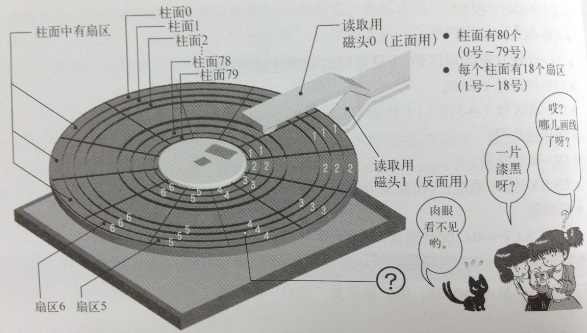
\includegraphics[width=0.6\textwidth]{day03-ruanpan.jpg}\\
  \caption{软盘的结构}\label{ruanpan}
\end{figure}

一张软盘有80个柱面,2个磁头,18个扇区,且一个扇区有512字节。所以一张软盘的容量是$80\times 2\times 18\times 512=1474560 Byte= 1440KB$。

含有IPL的启动区,位于C0-H0-S1(柱面0,磁头0,扇区1),下一个扇区是C0-H0-S2,这次我们要装载的扇区就是这个。

ES:BX=缓冲地址~是个内存地址,表明要把软盘上读出的数据装载到内存的哪个位置。由于一个BX只能表示0$\sim$0xffff的值,即64K,太小了,使用段寄存器以ES:BX这种方式来表示地址,写成“MOV AL,[ES:BX]”,代表“ES$\times$16+BX” 的内存地址。程序中指定了ES=0x0820,BX=0,所以软盘的数据会被装载到0x8200$\sim$0x83ff的位置。
\cs

作者使用变量的方式改写了Makefile文件,可以看一下。

\section{	试错	}
鉴于软盘的不可靠性,有时候需要在软盘读不出来的时候多读几次,这里重读5 次。

\dag|projects\03_day\harib00b|
\begin{code}[label=ipl.nas 本次添加的部分]
; ディスクを読む

		MOV		AX,0x0820
		MOV		ES,AX
		MOV		CH,0			; シリンダ0
		MOV		DH,0			; ヘッド0
		MOV		CL,2			; セクタ2

		MOV		SI,0			; 失敗回数を数えるレジスタ
retry:
		MOV		AH,0x02			; AH=0x02 : ディスク読み込み
		MOV		AL,1			; 1セクタ
		MOV		BX,0
		MOV		DL,0x00			; Aドライブ
		INT		0x13			; ディスクBIOS呼び出し
		JNC		fin				; エラーがおきなければfinへ
		ADD		SI,1			; SIに1を足す
		CMP		SI,5			; SIと5を比較
		JAE		error			; SI >= 5 だったらerrorへ
		MOV		AH,0x00
		MOV		DL,0x00			; Aドライブ
		INT		0x13			; ドライブのリセット
		JMP		retry
\end{code}

其中,JNC(jump if not carry),进位标志为0的话跳转;JAE(jump if above or equal),大于或等于时跳转。

在重新读盘之前,做了如下处理,AH=0x00,DL=0x00,INT=0x13,即完成系统复位。
\section{	读到18扇区	}
往后多读几个扇区,读完柱面0的18个扇区。

\dag|projects\03_day\harib00c|
\begin{code}[label=ipl.nas 本次添加的部分]
; ディスクを読む

		MOV		AX,0x0820
		MOV		ES,AX
		MOV		CH,0			; シリンダ0
		MOV		DH,0			; ヘッド0
		MOV		CL,2			; セクタ2
readloop:
		MOV		SI,0			; 失敗回数を数えるレジスタ
retry:
		MOV		AH,0x02			; AH=0x02 : ディスク読み込み
		MOV		AL,1			; 1セクタ
		MOV		BX,0
		MOV		DL,0x00			; Aドライブ
		INT		0x13			; ディスクBIOS呼び出し
		JNC		next			; エラーがおきなければnextへ
		ADD		SI,1			; SIに1を足す
		CMP		SI,5			; SIと5を比較
		JAE		error			; SI >= 5 だったらerrorへ
		MOV		AH,0x00
		MOV		DL,0x00			; Aドライブ
		INT		0x13			; ドライブのリセット
		JMP		retry
next:
		MOV		AX,ES			; アドレスを0x200進める
		ADD		AX,0x0020
		MOV		ES,AX			; ADD ES,0x020 という命令がないのでこうしている
		ADD		CL,1			; CLに1を足す
		CMP		CL,18			; CLと18を比較
		JBE		readloop		; CL <= 18 だったらreadloopへ
\end{code}

JBE(jump if below or equal),小于等于则跳转。

要读入下一个扇区只需给CL加1,给ES加上0x20(512/16)。CL是扇区号,ES指定读入地址。

这里使用循环的方式读入各个扇区,而不是在开始的时候设置读入的扇区数AL=17,因为磁盘BIOS读盘函数有一些“补充说明”:
\begin{quote}
  指定处理的扇区数,范围在0x01~0xff(指定0x02以上的数值时,要特别注意能够连续处理多个扇区的条件。如果是FD的话,似乎不能跨越多个磁道,也不能超过64KB的界限。)
\end{quote}

经过上面这些读盘处理,已经把磁盘上C0-H0-S2到C0-H0-S18的$512\times 17=8704$个字节的内容,装载到了内存的0x8200$\sim$0xa3ff。
\section{	读入10个柱面	}
C0-H0-S18扇区的下一个扇区是磁盘反面的C0-H1-S1,按顺序读到C0-H1-S18,接着读C1-H0-S1,最后一直读到C9-H1-S18。

\dag |projects\03_day\harib00d|
\begin{code}
; ディスクを読む

		MOV		AX,0x0820
		MOV		ES,AX
		MOV		CH,0			; シリンダ0
		MOV		DH,0			; ヘッド0
		MOV		CL,2			; セクタ2
readloop:
		MOV		SI,0			; 失敗回数を数えるレジスタ
retry:
		MOV		AH,0x02			; AH=0x02 : ディスク読み込み
		MOV		AL,1			; 1セクタ
		MOV		BX,0
		MOV		DL,0x00			; Aドライブ
		INT		0x13			; ディスクBIOS呼び出し
		JNC		next			; エラーがおきなければnextへ
		ADD		SI,1			; SIに1を足す
		CMP		SI,5			; SIと5を比較
		JAE		error			; SI >= 5 だったらerrorへ
		MOV		AH,0x00
		MOV		DL,0x00			; Aドライブ
		INT		0x13			; ドライブのリセット
		JMP		retry
next:
		MOV		AX,ES			; アドレスを0x200進める
		ADD		AX,0x0020
		MOV		ES,AX			; ADD ES,0x020 という命令がないのでこうしている
		ADD		CL,1			; CLに1を足す
		CMP		CL,18			; CLと18を比較
		JBE		readloop		; CL <= 18 だったらreadloopへ
		MOV		CL,1
		ADD		DH,1
		CMP		DH,2
		JB		readloop		; DH < 2 だったらreadloopへ
		MOV		DH,0
		ADD		CH,1
		CMP		CH,CYLS
		JB		readloop		; CH < CYLS だったらreadloopへ
\end{code}

JB(jump if below),如果小于就跳转。

在程序开头使用了EQU指令来声明常数,即|CYLS EQU 10|。
现在已经能够把软盘最初的$10\times 2\times 18\times512=184320 byte= 180KB $的内容完整的装载到内存中了。

\section{	着手开发操作系统	}
编写一个短小的程序,只让它HLT。

\dag |projects\03_day\harib00e|
\begin{code}[label=haribote.nas]
fin:
    HLT
    JMP fin
\end{code}

使用nask编译,输出成harbote.sys。用“make img”指令来生成映像文件。

使用作者最开始提到的二进制编辑器查看haribote.img 和haribote.sys内容,可以发现0x002600附近保存着文件名,0x004200位置保存着文件的内容,这里分别是haribotesys 和编译后的harbote.sys里面的内容“|F4 EB FD|”。

这样,要做的工作就是将操作系统的本身的内容写到名为harbote.sys的问卷中,再把它保存到磁盘映像里,然后从启动区执行这个harbote.sys 就行了。
\section{	从启动区执行操作系统	}
现在的程序是从启动区开始,把磁盘上的内容装载到内存 0x8000 号地址,所以磁盘映像上位于 0x004200 号地址的程序位于内存的0x8000+0x4200=0xc200号地址。

修改haribote.nas,加上ORG 0xc200,然后在ipl.nas处理的最后加上JMP 0xc200这个指令。详细程序见“projects/03\_day/harib00f”。

通过运行“make run”来运行程序。
\section{	确认操作系统的执行情况	}
通过切换以下画面模式,让画面变成一片漆黑,证明程序正常运行。

\dag |projects/03_day/harib00g|

\begin{code}
; haribote-os
; TAB=4

		ORG		0xc200			; このプログラムがどこに読み込まれるのか

		MOV		AL,0x13			; VGAグラフィックス、320x200x8bitカラー
		MOV		AH,0x00
		INT		0x10
fin:
		HLT
		JMP		fin
\end{code}

设置显卡模式:
\begin{itemize}
  \item AH=0x00
  \item AL=模式:
  \begin{itemize}
    \item 0x03:16色字符模式,80$\times$25
    \item 0x12:VGA图形模式,640$\times$480$\times$4位彩色模式,独特的4面存储模式
    \item 0x13:VGA图形模式,320$\times$200$\times$8位彩色模式,调色板模式
    \item 扩展VGA图形模式,800$\times$600$\times$4位彩色模式,独特的4面存储模式
  \end{itemize}
  \item 返回值:无
\end{itemize}

程序的变动:
将ipl.nas改名为ipl10.nas,提醒这个程序只能读入10个柱面。

想把磁盘装载内容的结束地址告诉给haribote.sys,在ipl10.nas文件中“JMP 0xc200”之前加入了一行代码,将CYLS的值写到内存地址0x0ff0中。

运行“make run”查看效果,应该是一片漆黑画面。

\section[32位模式前期准备]{32位模式前期准备\protect\footnote{书中作者先讲述了为什么用32位模式,自己看下书吧。}}

考虑到系统以后会支持各种不同的画面模式,就需要把现在的设置信息(BOOT\_INFO)保存起来以备后用。

\dag|projects\03_day\harib00h|
\begin{code}[label=haribote.nas]
; haribote-os
; TAB=4

; BOOT_INFO関係
CYLS	EQU		0x0ff0			; ブートセクタが設定する
LEDS	EQU		0x0ff1
VMODE	EQU		0x0ff2			; 色数に関する情報。何ビットカラーか?
SCRNX	EQU		0x0ff4			; 解像度のX
SCRNY	EQU		0x0ff6			; 解像度のY
VRAM	EQU		0x0ff8			; グラフィックバッファの開始番地

		ORG		0xc200			; このプログラムがどこに読み込まれるのか

		MOV		AL,0x13			; VGAグラフィックス、320x200x8bitカラー
		MOV		AH,0x00
		INT		0x10
		MOV		BYTE [VMODE],8	; 画面モードをメモする
		MOV		WORD [SCRNX],320
		MOV		WORD [SCRNY],200
		MOV		DWORD [VRAM],0x000a0000

; キーボードのLED状態をBIOSに教えてもらう

		MOV		AH,0x02
		INT		0x16 			; keyboard BIOS
		MOV		[LEDS],AL

fin:
		HLT
		JMP		fin
\end{code}

|[VRAM]|里保存的是 0xa0000。VRAM是显卡内存,它的各个地址对应画面上的像素。不同的画面模式对应不同的VRAM,因此这里将使用的VRAM地址保存在BOOT\_INFO里。这种画面模式下VRAM是“0xa000$\sim$0xaffff的64KB”。画面的像素数、颜色数以及从BIOS取得的键盘信息都保存在内存0x0ff0位置附近。


\section{	开始导入C语言	}

现在,直接切换到32位模式,然后运行C语言写程序。

程序做了很大的改动,haribote.sys的前半部分使用汇编语言编写的,后半部分是用C语言编写的,所以将haribote.nas改成了asmhead.nas,并且,为了调用C 语言写的程序,添加了100行左右的汇编代码。这些汇编代码作者在后面再讲解,这里直接跳过,分析C语言部分。

C语言部分写在bootpack.c文件中。

\dag|projects\03_day\harib00i|
\begin{code}[label=bootpack.c]
void HariMain(void)
{

fin:
	/* ここにHLTを入れたいのだが、C言語ではHLTが使えない! */
	goto fin;

}
\end{code}

\cs

bootpack.c变成机器语言的过程:
\begin{enumerate}
  \item 使用ccl.exe从bootpack.c生成bootpack.gas;
  \item 使用gas2nask.exe从 bootpack.gas生成bootpack.nas;
  \item 使用nask.exe从bootpack.nas生成bootpack.obj;
  \item 使用obj2bim.exe从bootpack.obj生成bootpack.bim;
  \item 使用bim2hrb.exe从bootpack.bim生成bootpack.hrb;
  \item 使用copy指令将asmhead.bin与bootpack.hrb单纯结合起来就生成了haribote.sys。
\end{enumerate}

\section{	实现HLT(harib00j)	}

\dag|projects\03_day\harib00j|
\begin{code}[label=naskfun.nas]
; naskfunc
; TAB=4

[FORMAT "WCOFF"]				; オブジェクトファイルを作るモード	
[BITS 32]						; 32ビットモード用の機械語を作らせる


; オブジェクトファイルのための情報

[FILE "naskfunc.nas"]			; ソースファイル名情報

		GLOBAL	_io_hlt			; このプログラムに含まれる関数名


; 以下は実際の関数

[SECTION .text]		; オブジェクトファイルではこれを書いてからプログラムを書く

_io_hlt:	; void io_hlt(void);
		HLT
		RET
\end{code}

使用汇编语言编写了一个函数,io\_hlt。将输出设置为WCOFF模式,可以编译成目标文件,与bootpack.obj链接。

在nask目标文件的模式下,必须设定文件名信息,然后再写明下面程序的函数名。需要先在函数名前面加上“\_”,否则不能很好地与C语言函数链接。需要链接的函数名都需要GLOBAL指令声明。

下面写一个实际的函数。先写一个与用GLOBAL声明的函数名相同的标号,从此处开始写代码就可以了。

\dag|projects\03_day\harib00j|
\begin{code}[label=bootpack.c]
/* 他のファイルで作った関数がありますとCコンパイラに教える */

void io_hlt(void);

/* 関数宣言なのに、{}がなくていきなり;を書くと、
	他のファイルにあるからよろしくね、という意味になるのです。 */

void HariMain(void)
{

fin:
	io_hlt(); /* これでnaskfunc.nasの_io_hltが実行されます */
	goto fin;

}
\end{code}


“make run”运行程序。
